\documentclass[a4paper,twoside]{article}
\usepackage[T1]{fontenc}
\usepackage[bahasa]{babel}
\usepackage{graphicx}
\usepackage{graphics}
\usepackage{float}
\usepackage[cm]{fullpage}
\pagestyle{myheadings}
\usepackage{etoolbox}
\usepackage{setspace} 
\usepackage{lipsum} 
\usepackage{algorithm}
\usepackage{algorithmic}
\usepackage{tabularx}
\usepackage{amsmath}
\usepackage{listings}
\usepackage{pgffor}% untuk foreach
\usepackage[table]{xcolor}%untuk kode program
\setlength{\headsep}{30pt}
\usepackage[inner=2.5cm,outer=2.5cm,top=2.5cm,bottom=2cm]{geometry} %margin
% \pagestyle{empty}

\makeatletter
\renewcommand{\@maketitle} {\begin{center} {\LARGE \textbf{ \textsc{\@title}} \par} \bigskip {\large \textbf{\textsc{\@author}} }\end{center} }
\renewcommand{\thispagestyle}[1]{}
\markright{\textbf{\textsc{Laporan Perkembangan Pengerjaan Skripsi\textemdash Sem. Ganjil 2018/2019}}}

\onehalfspacing
 
\begin{document}

\title{\@judultopik}
\author{\nama \textendash \@npm} 

%ISILAH DATA BERIKUT INI:
\newcommand{\nama}{Cornelius David Herianto}
\newcommand{\@npm}{2015730034}
\newcommand{\tanggal}{15/11/2018} %Tanggal pembuatan dokumen
\newcommand{\@judultopik}{Pengelompokan Dokumen Berbasis Algoritma Genetika} % Judul/topik anda
\newcommand{\kodetopik}{TAB4502}
\newcommand{\jumpemb}{1} % Jumlah pembimbing, 1 atau 2
\newcommand{\pembA}{Thomas Anung Basuki}
\newcommand{\pembB}{-}
\newcommand{\semesterPertama}{45 - Ganjil 18/19} % semester pertama kali topik diambil, angka 1 dimulai dari sem Ganjil 96/97
\newcommand{\lamaSkripsi}{1} % Jumlah semester untuk mengerjakan skripsi s.d. dokumen ini dibuat
\newcommand{\kulPertama}{Skripsi 1} % Kuliah dimana topik ini diambil pertama kali
\newcommand{\tipePR}{C} % tipe progress report :
% A : dokumen pendukung untuk pengambilan ke-2 di Skripsi 1
% B : dokumen untuk reviewer pada presentasi dan review Skripsi 1
% C : dokumen pendukung untuk pengambilan ke-2 di Skripsi 2

% Dokumen hasil template ini harus dicetak bolak-balik !!!!

\maketitle

\pagenumbering{arabic}

\section{Data Skripsi} %TIDAK PERLU MENGUBAH BAGIAN INI !!!
Pembimbing utama/tunggal: {\bf \pembA}\\
Pembimbing pendamping: {\bf \pembB}\\
Kode Topik : {\bf \kodetopik}\\
Topik ini sudah dikerjakan selama : {\bf \lamaSkripsi} semester\\
Pengambilan pertama kali topik ini pada : Semester {\bf \semesterPertama} \\
Pengambilan pertama kali topik ini di kuliah : {\bf \kulPertama} \\
Tipe Laporan : {\bf \tipePR} -
\ifdefstring{\tipePR}{A}{
			Dokumen pendukung untuk {\BF pengambilan ke-2 di Skripsi 1} }
		{
		\ifdefstring{\tipePR}{B} {
				Dokumen untuk reviewer pada presentasi dan {\bf review Skripsi 1}}
			{	Dokumen pendukung untuk {\bf pengambilan ke-2 di Skripsi 2}}
		}
		
\section{Latar Belakang}
Pengelompokan (\textit{clustering}) merupakan teknik yang digunakan untuk membagi kumpulan data (\textit{dataset}) ke dalam kelompok objek serupa. Setiap kelompok (\textit{cluster}) terdiri dari objek-objek yang serupa satu sama lain berdasarkan suatu ukuran dan tidak serupa dengan objek-objek lain di luar kelompoknya.

\textit{Clustering} merupakan salah satu teknik pembelajaran tak terarah (\textit{unsupervised learning}). Pembagian kelompok dalam \textit{clustering} tidak berdasarkan sesuatu yang telah diketahui sebelumnya, melainkan berdasarkan kesamaan tertentu menurut suatu ukuran tertentu.

Salah satu algoritma pengelompokan yang paling sering digunakan adalah \textit{K-means} yang dilakukan dengan cara membagi data ke dalam \textit{K} kelompok. Kelompok tersebut dibentuk dengan cara meminimalkan jarak antara titik pusat \textit{cluster} (\textit{centroid}) dengan setiap anggota \textit{cluster} tersebut. Titik pusat \textit{cluster} dicari dengan menggunakan rata-rata (\textit{mean}) dari nilai setiap anggota \textit{cluster}. Dalam hal ini, setiap anggota \textit{cluster} dimodelkan sebagai vektor dalam $n$ dimensi ($n$ merupakan banyaknya atribut). \textit{K-means} sudah terbukti efektif dalam melakukan pengelompokan  dalam situasi apapun. Namun, cara tersebut tetap saja memiliki kekurangan yaitu dapat terjebak dalam \textit{local optima} tergantung dengan pemilihan \textit{centroid} awal.

Masalah \textit{local optima} dapat ditangani menggunakan \textit{Genetic Algorithm} (GA) yang telah terbukti efektif dalam menyelesaikan masalah pencarian dan optimasi. GA merupakan teknik pencarian heuristik tingkat tinggi yang menirukan proses evolusi yang secara alami terjadi berdasarkan prinsip \textit{survival of the fittest}. Algoritma ini dinamakan demikian karena menggunakan konsep-konsep dalam genetika sebagai model pemecahan masalahnya. 

Dalam GA, parameter dari \textit{search space} dikodekan dalam bentuk deretan objek yang disebut kromosom. Kumpulan kromosom tersebut lalu dikenal sebagai populasi. Pada awalnya, populasi dibangkitkan secara acak. Kemudian, akan dipilih beberapa kromosom menggunakan teknik \textit{roulette wheel selection} berdasarkan fungsi \textit{fitness}. Operasi dasar yang terinspirasi dari Ilmu Biologi seperti persilangan (\textit{crossover}) dan mutasi (\textit{mutation}) digunakan untuk membangkitkan generasi berikutnya. Proses seleksi, persilangan, dan mutasi ini berlangsung dalam jumlah generasi tertentu atau sampai kondisi akhir tercapai.

Fungsi \textit{fitness} tidak hanya berfungsi untuk menentukan seberapa baik solusi yang dihasilkan namun juga menentukan seberapa dekat solusi tersebut dengan hasil yang optimal. Oleh karena itu, diperlukan fungsi \textit{fitness} yang cocok sehingga GA dapat menghasilkan keluaran yang optimal. Pada masalah \textit{clustering} menggunakan GA, maka fungsi \textit{fitness} yang digunakan harus bisa menggambarkan bahwa seluruh elemen sudah berada dalam \textit{cluster} yang terbaik dan sudah sesuai.

\section{Rumusan Masalah}
Berdasarkan latar belakang yang telah dipaparkan, rumusan masalah dari penelitian ini adalah sebagai berikut:

\begin{enumerate}
 \item Bagaimana algoritma genetik dapat digunakan untuk mengelompokkan dokumen?
 \item Bagaimana membangun perangkat lunak yang menggunakan algoritma genetik untuk dapat mengelompokkan
dokumen?
\end{enumerate}

\section{Tujuan}
Berdasarkan rumusan masalah yang telah disebutkan, tujuan dari penelitian ini adalah sebagai berikut:

\begin{enumerate}
	\item Mempelajari algoritma genetik dan hubungannya dengan pengelompokan dokumen.
	\item Membangun perangkat lunak yang mengimplementasikan algoritma genetik untuk dapat mengelompokkan
dokumen.
\end{enumerate}

\section{Detail Perkembangan Pengerjaan Skripsi}
Detail bagian pekerjaan skripsi sesuai dengan rencan kerja/laporan perkembangan terkahir :
	\begin{enumerate}
		\item \textbf{Melakukan studi literatur mengenai {\it Information Retrieval} (temu kembali informasi).}\\
		{\bf Status :} Baru ditambahkan semester ini\\
		{\bf Hasil :} Temu kembali informasi adalah bidang ilmu yang berurusan dengan representasi, penyimpanan, pengolahan, dan akses terhadap informasi. Pada penelitian ini, temu kembali informasi memiliki peran untuk mengubah dokumen yang semula berbentuk teks menjadi sesuatu yang memiliki nilai informasi agar nantinya bisa diproses lebih lanjut (dalam kasus ini dengan pengelompokan dokumen).

Dalam penelitian ini, temu kembali informasi digunakan untuk merepresentasikan dokumen ke dalam model ruang vektor agar bisa dilakukan pengelompokan. Tahap pertama yang dilakukan adalah membentuk kosa kata (\textit{vocabulary}) yang berisi seluruh istilah berbeda yang ada di setiap dokumen yang akan diindeks. Kemudian, untuk setiap dokumen akan dibentuk suatu indeks yang terdiri dari pasangan antara istilah di dokumen tersebut dan jumlah kemunculannya (\textit{term-document incidence matrix}). Tabel \ref{tbl:term-doc} merupakan contoh dari \textit{term-document incidence matrix} dengan baris pada tabel menunjukkan istilah (\textit{term}) dan kolom menunjukkan nama dokumen. Sel bernilai $1$ apabila dokumen mengandung term tertentu dan $0$ jika tidak.

Selanjutnya, setiap jumlah kemunculan suatu istilah dalam sebuah dokumen akan diubah menjadi suatu bobot tertentu berdasarkan teknik pemodelannya. Dalam penelitian ini, digunakan 2 teknik pembobotan yaitu bobot frekuensi dan bobot tf-idf.

\subsection*{Bobot frekuensi}
Bobot frekuensi merupakan teknik pembobotan yang sangat sederhana karena bobotnya merupakan jumlah kemunculan istilah tersebut dalam dokumen. Bobot frekuensi dapat digambarkan dalam rumus:
\begin{equation}
w_i=tf_i
\end{equation}
dengan $w_i$ merupakan bobot istilah ke-$i$ dan $tf_i$ merupakan frekuensi kemunculan istilah ke-$i$ pada dokumen.

\begin{table}[h]
\label{tbl:term-doc}
\centering
\begin{tabular}{lccccccc}
& \begin{tabular}[c]{@{}c@{}}Anthony\\ and \\ Cleopatra\end{tabular} & \begin{tabular}[c]{@{}c@{}}Julius \\ Caesar\end{tabular} & \begin{tabular}[c]{@{}c@{}}The \\ Tempest\end{tabular} & Hamlet & Othello & Macbeth & ... \\
Anthony		& 1 & 1 & 0 & 0 & 0 & 1 & \\
Brutus 		& 1 & 1 & 0 & 1 & 0 & 0 & \\
Caesar 		& 1 & 1 & 0 & 1 & 1 & 1 & \\
Calpurnia 	& 0 & 1 & 0 & 0 & 0 & 0 & \\
Cleopatra 	& 1 & 0 & 0 & 0 & 0 & 0 & \\
mercy 		& 1 & 0 & 1 & 1 & 1 & 1 & \\
worser 		& 1 & 0 & 1 & 1 & 1 & 0 & \\
...  
\end{tabular}
\caption{\textit{Term-document incidence matrix}}
\end{table}

\subsection*{Bobot TF-IDF}
Pada bobot frekuensi, bobot hanya dihitung berdasarkan kemunculan istilah dalam dokumen itu sendiri. Namun dalam bobot TF-IDF (\textit{term frequency-inverse document frequency}), bobot juga dihitung berdasarkan kemunculan istilah pada himpunan dokumen. Metode ini sangat populer digunakan oleh sistem rekomendasi berbasis teks. Rumus dari TF-IDF adalah sebagai berikut: 
\begin{equation}
w_i=tf_i \times log \frac{N}{N_i}
\end{equation}
dengan $w_i$ merupakan bobot istilah ke-$i$, $tf_i$ merupakan frekuensi kemunculan istilah ke-$i$ pada dokumen, $N$ menyatakan banyaknya anggota himpunan dokumen, dan $N_i$ menunjukkan frekuensi dokumen dari istilah ke-$i$ (banyaknya dokumen pada himpunan dokumen yang memuat istilah ke-$i$).

Berdasarkan rumus tersebut, maka dapat ditarik dua kesimpulan yaitu:
\begin{itemize}
\item Semakin sering suatu istilah muncul di suatu dokumen, maka semakin representatif istilah tersebut terhadap isi dokumen.
\item Semakin banyak dokumen yang memuat suatu istilah, maka nilai informasi istilah tersebut semakin kecil.
\end{itemize}

Metode penetapan bobot TF-IDF dianggap sebagai metode yang berkinerja baik karena mempertimbangkan frekuensi kemunculan istilah baik secara lokal (TF) maupun global (IDF).


\subsection*{Model ruang vektor}
Model ruang vektor adalah representasi dari koleksi dokumen sebagai vektor dalam ruang vektor yang umum. Model ruang vektor ini biasanya digunakan dalam sejumlah operasi pencarian informasi mulai dari penilaian dokumen pada \textit{query}, klasifikasi dokumen dan pengelompokan dokumen.

Dalam pengolahan model ruang vektor, dibutuhkan cara untuk menghitung kesamaan antara dua ruang vektor. Dalam pengelompokan dokumen, apabila kesamaan antara dua buah vektor semakin besar, maka peluang kedua vektor tersebut berada dalam sebuah kelompok yang sama akan semakin besar. Dalam penelitian ini, digunakan dua cara untuk menghitung kesamaan antara dua ruang vektor yaitu menggunakan Jarak Euclidean (\textit{Euclidean distance}) dan persamaan cosinus (\textit{cosine similarity}).

\subsubsection*{Jarak Euclidean}
\label{sub:euclideanDist}
Jarak Euclidean atau biasa disebut jarak garis lurus merupakan metode paling banyak digunakan untuk menghitung jarak antara dua buah vektor. Secara umum, rumus dari Jarak Euclidean adalah sebagai berikut:
\begin{equation}
d_{ij}=\sqrt{\sum_{v=1}^N (x_{vi}-x_{vj})^2}
\end{equation}
dengan $d_{ij}$ adalah jarak antara vektor ke-$i$ dengan vektor ke-$j$, $N$ adalah jumlah dimensi pada vektor, dan $x_{vi}$ adalah nilai dimensi ke-$v$ dari vektor ke-$i$.

\subsubsection*{Persamaan Cosinus}
\label{sub:cosineDist}
Persamaan cosinus merupakan normalisasi hasil kali titik dengan panjang masing-masing vektor. Persamaan cosinus memiliki persamaan sebagai berikut:
\begin{equation}
s_{ij}=\frac{i\cdot j}{\parallel i \parallel \times \parallel j \parallel}
\end{equation}
dengan $s_{ij}$ adalah kesamaan antara vektor ke-$i$ dengan vektor ke-$j$, $i$ adalah vektor ke-$i$, dan $j$ adalah vektor ke-$j$. Persamaan ini menjelaskan bahwa semakin kecil sudut antara dua vektor, maka tingkat kemiripannya semakin besar.
		
		\item \textbf{Melakukan studi literatur mengenai {\it Document Clustering} (pengelompokan dokumen).}\\
		{\bf Status :} Ada sejak rencana kerja skripsi\\
		{\bf Hasil :} Tugas pengelompokan (\textit{clustering}) merupakan salah satu bagian dari pembelajaran mesin. Pengelompokan terdiri dari dua jenis berdasarkan metode pembelajarannya. \textit{Classification} merupakan jenis pembelajaran terarah karena sudah diberikan label sejak awal, lalu dilakukan pengelompokan berdasarkan label untuk setiap kelompoknya. Sedangkan \textit{clustering} merupakan jenis pembelajaran tak terarah karena tidak diberikan label sejak awal sehingga pengelompokan dilakukan berdasarkan suatu kesamaan tertentu.

\subsection*{K-Means}
K-means merupakan algoritma pengelompokan yang paling populer digunakan saat ini. algoritma ini membagi data ke dalam $K$ \textit{cluster}. Setiap \textit{cluster} direpresentasikan dengan titik tengahnya (\textit{centroid}). Setiap iterasi, titik tengah akan dihitung sebagai rata-rata dari semua titik data dari \textit{cluster} tersebut. Rumus untuk menghitung \textit{centroid} adalah sebagai berikut:
\begin{equation}
\label{eq:kmeans}
\mu_i=\frac{1}{N_i}\sum_{q=1}^{N_i}x_q
\end{equation}
dengan $\mu_i$ merupakan \textit{centroid} ke-$i$, $N_i$ merupakan jumlah titik data pada \textit{cluster} ke-$i$, dan $x_q$ merupakan titik ke-$q$ pada \textit{cluster} ke-$i$.

\begin{algorithm} % enter the algorithm environment
\caption{K-Means} % give the algorithm a caption
\label{alg:kmeans} % and a label for \ref{} commands later in the document
\begin{flushleft}
	\textbf{Input:} $S$ (himpunan titik data), $K$ (Jumlah \textit{cluster})\\
	\textbf{Output:} himpunan \textit{cluster}
\end{flushleft}
\begin{algorithmic}[1] % enter the algorithmic environment
	\STATE Pilih $K$ titik data sebagai himpunan awal \textit{centroid}.
	\REPEAT 
		\STATE Bentuk $K$ \textit{cluster} dengan menempatkan setiap titik data ke \textit{cluster} dengan \textit{centroid} terdekat.
		\STATE Hitung ulang \textit{centroid} untuk setiap \textit{cluster}. 
	\UNTIL{\textit{Centroid} tidak berubah.}
\end{algorithmic}
\end{algorithm}

Algoritma K-means diawali dengan penentuan \textit{centroid} secara acak. Pada setiap iterasi, setiap data ditetapkan pada \textit{cluster} yang memiliki \textit{centroid} dengan jarak terdekat dari titik data tersebut, kemudian posisi \textit{centroid} dari setiap \textit{cluster} akan dihitung ulang dengan Persamaan \ref{eq:kmeans}. Iterasi akan terus diulang sampai posisi dari semua \textit{cluster} tidak berubah.
		
    	\item \textbf{Melakukan studi literatur mengenai {\it Genetic Algorithm} (algoritma genetik).}\\
    	{\bf Status :} Ada sejak rencana kerja skripsi\\
		{\bf Hasil :} Algoritma genetika (GA) adalah suatu algoritma pencarian yang terinspirasi dari proses seleksi alam yang terjadi secara alami dalam proses evolusi. Ada beberapa istilah yang digunakan dalam algoritma genetika di antaranya kromosom, seleksi, persilangan, mutasi, dan fungsi \textit{fitness}.

\subsection*{Kromosom}
\label{sub:chromosome}
Dalam GA, kromosom adalah himpunan parameter yang mendefinisikan suatu solusi yang diusulkan. Kromosom biasanya direpresentasikan sebagai string yang berisi kumpulan nilai (gen), meskipun berbagai struktur data lainnya juga digunakan.

\subsection*{Seleksi}
\label{sub:selection}
Seleksi dalam algoritma genetika bertugas untuk memilih kromosom dari populasi untuk proses persilangan. Salah satu teknik yang populer digunakan dalam seleksi adalah \textit{roulette-wheel selection}. Teknik ini memungkinkan terjadinya pemilihan berdasarkan fungsi \textit{fitness} sehingga kromosom yang memiliki fungsi \textit{fitness} lebih besar memiliki peluang lebih besar untuk terpilih dan menjadi induk dari generasi selanjutnya.

\subsection*{Persilangan}
\label{sub:crossover}
Persilangan adalah operasi genetik yang digunakan untuk menggabungkan informasi genetik dari dua induk untuk menghasilkan keturunan baru. Teknik persilangan yang digunakan dalam penelitian ini adalah \textit{Single-point crossover}. Dalam teknik ini, sebuah titik pada kedua induk dipilih untuk menjadi titik persilangan (\textit{crossover point}). Bit yang berada di sebelah kanan titik persilangan bertukar antara kedua kromosom induk seperti yang ditunjukkan pada Gambar \ref{fig:spcrossover}.

\begin{figure}[h]
	\begin{center}
		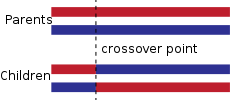
\includegraphics{OnePointCrossover}
		\caption{\textit{Single-point crossover}}
		\label{fig:spcrossover}
	\end{center}
\end{figure}

\subsection*{Mutasi}
\label{sub:mutation}
Mutasi adalah suatu operator genetik yang digunakan untuk mempertahankan keragaman genetik dari satu generasi populasi dalam algoritma genetika. Mutasi mengubah satu atau beberapa nilai dalam gen. Mutasi terjadi berdasarkan probabilitas mutasi yang sudah ditentukan sebelumnya. Probabilitas ini seharusnya bernilai kecil, karena jika terlalu besar maka akan menjadi sama dengan algoritma pencarian acak primitif (\textit{primitive random search}). Pada penelitian ini, kromosom memiliki gen yang bernilai non-biner. Oleh karena itu, mutasi dilakukan dengan memilih sebuah bilangan acak antara batas bawah dan batas atas nilai suatu gen.

\subsection*{Fungsi \textit{Fitness}}
\label{sub:fitnessFn}
Fungsi \textit{fitness} adalah fungsi objektif yang digunakan untuk mengukur seberapa baik suatu kromosom sebagai calon solusi. Sebuah fungsi \textit{fitness} harus bisa memperkirakan seberapa dekat sebuah calon solusi dengan solusi yang optimal. Dalam algoritma genetika, fungsi \textit{fitness} juga digunakan dalam proses seleksi (\textit{roulette-wheel selection}) untuk menentukan seberapa baik suatu kromosom untuk menjadi induk dari generasi berikutnya.

\begin{algorithm}[h]
	\caption{Algoritma Genetika}
	\label{alg:GA}
	\begin{flushleft}
		\textbf{function} Algoritma-Genetika(\textit{populasi},Fung-Fitness) \textbf{returns} solusi berupa individu
		\begin{flushleft}
			\begin{tabular}{ l l }
  				\textbf{inputs:} & \textit{populasi}, himpunan individu \\
 		 		& Fung-Fitness, fungsi yang mengukur \textit{fitness} dari tiap individu
			\end{tabular}
			\hspace{5pt}  
		\end{flushleft}
	\end{flushleft}
	\begin{algorithmic}[1]
		\REPEAT
			\STATE $populasi\_baru \leftarrow$ himpunan kosong
			\FOR{$i$=1 \TO Size($populasi$)} 
				\STATE $x \leftarrow$ Seleksi-acak(populasi, Fung-Fitness)
				\STATE $y \leftarrow$ Seleksi-acak(populasi, Fung-Fitness)
				\STATE $anak \leftarrow$ Persilangan($x$, $y$)
				\IF{probabilitas mutasi} 
					\STATE Mutasi($anak$)
				\ENDIF
				\STATE tambahkan $anak$ ke $populasi\_baru$
			\ENDFOR
			\STATE $populasi \leftarrow populasi\_baru$
		\UNTIL{kriteria berakhir dipenuhi atau sampai jumlah generasi tertentu}
		\RETURN {individu terbaik dalam populasi, berdasarkan Fung-Fitness}
	\end{algorithmic}

	\rule{\textwidth}{0.4pt}
	\begin{flushleft}
		\textbf{function} Persilangan($x$,$y$) \textbf{returns} anak berupa individu
		\begin{flushleft}
			\begin{tabular}{ l l }
				\textbf{inputs:}& $x$, $y$, individu induk
				\hspace{5pt} 
			\end{tabular} 
		\end{flushleft}
	\end{flushleft}
	
	\begin{algorithmic}[1]
		\STATE $n \leftarrow$ Length($x$)
		\STATE $c \leftarrow$ angka acak antara 1 sampai $n$
		\RETURN{Append(Substring($x$,1,$c$), Substring($y$,$c$+1,$n$))}
	\end{algorithmic}
	\hspace{5pt} 
\end{algorithm}

\subsection*{Proses pencarian dalam algoritma genetika}
Seperti yang disebutkan dalam Algoritma \ref{alg:GA}, algoritma genetika dimulai dengan menginisialisasi suatu populasi (biasanya dibangkitkan secara acak jika tidak diketahui heuristik masalahnya). Lalu, akan dibangkitkan populasi baru untuk generasi berikutnya dengan cara mengambil dua kromosom secara acak dengan teknik \textit{roulette-wheel selection}. Setelah itu akan dilakukan persilangan dengan teknik \textit{single-point crossover}. Teknik ini dilakukan dengan cara menentukan sebuah titik potong $c$ yang diambil secara acak antara angka 1 sampai panjang kromosom $n$. Keturunan dari kedua induk tersebut akan memiliki kromosom induk pertama dari gen ke-1 sampai gen ke-$c$ dan dari induk kedua mulai dari gen ke-($c$+1) sampai gen ke-$n$. Setelah itu, untuk apabila terjadi mutasi, maka salah satu gen dari anak akan diubah nilainya. Iterasi ini akan dilakukan terus-menerus hingga kriteria berhenti tercapai atau sudah mencapai batas jumlah generasi tertentu.
		
    	\item \textbf{Mempelajari penggunaan algoritma genetik dalam pengelompokan dokumen.}\\
    	{\bf Status :} Ada sejak rencana kerja skripsi\\
		{\bf Hasil :} Meskipun pada umumnya algoritma \textit{K-means} digunakan dalam pengelompokan, tetapi ternyata algoritma \textit{K-means} masih memiliki kekurangan yaitu masih dapat terjebak pada \textit{local optimum}. Oleh karena itu, pada penelitian ini digunakan algoritma genetika sebagai solusi dari permasalahan \textit{local optimum}. Algoritma genetika memiliki kemampuan untuk menghindari terjadinya \textit{local optimum} karena algoritma genetika merupakan algoritma pencarian yang bersifat stokastik karena memperbolehkan terjadinya variasi acak dalam proses pencarian solusinya. Oleh karena itu, diharapkan pengelompokan berbasis GA dapat menghasilkan solusi yang lebih baik dibandingkan dengan pengelompokan pada umumnya yang menggunakan algoritma \textit{K-means}.
		
    	\item \textbf{Mencari dokumen yang akan dijadikan {\it training} dan {\it test datasets}.}
    	{\bf Status :} Ada sejak rencana kerja skripsi\\
		{\bf Hasil :} Belum dikerjakan.
		
		\item \textbf{Melakukan analisis masalah dan mencari solusinya.}\\
    	{\bf Status :} Baru ditambahkan semester ini\\
		{\bf Hasil :} Untuk menyelesaikan masalah pengelompokan dokumen menggunakan algoritma genetika, maka perlu dibangun sebuah model yang dapat diterapkan ke dalam algoritma tersebut.
		
\subsection*{Representasi Kromosom}
Setiap \textit{string} kromosom merupakan deretan bilangan riil yang merepresentasikan $K$ titik pusat \textit{cluster} (\textit{centroid}). Dalam ruang $N$ dimensi, panjang dari kromosom akan menjadi $N\times K$ gen. $N$ kata pertama merepresentasikan $N$ dimensi dari \textit{centroid} pertama, $N$ kata selanjutnya merepresentasikan $N$ dimensi dari \textit{centroid} kedua, dan seterusnya.

\subsection*{Fungsi \textit{Fitness}}
Perhitungan \textit{fitness} dalam penelitian ini terdiri dari dua tahap. Pada tahap pertama, terjadi pembentukan \textit{cluster} berdasarkan titik pusat yang terkandung dalam kromosom. Hal ini dilakukan dengan menetapkan setiap titik $x_i,i=1,2, ... ,n$ ke dalam sebuah \textit{cluster} $C_j$ dengan \textit{centroid} $z_j$ sehingga

\begin{equation}
\Vert x_i-z_j \Vert < \Vert x_i-z_p \Vert , p=1,2, ... ,K \mbox{, dan } p \neq j.
\end{equation}

Setelah proses pengelompokan selesai, titik pusat yang terkandung dalam kromosom diganti dengan rata-rata titik dari tiap \textit{cluster}. Dengan kata lain, untuk \textit{cluster} $C_i$, \textit{centroid} baru $z_i^*$ dapat dihitung dengan rumus:

\begin{equation}
z_i^*=\frac{1}{n_i} \sum_{x_j\in C_i} x_j,   i=1,2, ... ,K.
\end{equation}

dengan $z_i^*$ merupakan titik pusat \textit{cluster} ke-$i$, $n_i$ merupakan jumlah anggota \textit{cluster} ke-$i$, dan $x_j$ merupakan titik ke-$j$ yang merupakan anggota dari \textit{cluster} ke-$i$. $z_i^*$ ini akan menggantikan $z_i$ sebelumnya di kromosom. Ada dua metode perhitungan fungsi fitness yang diimplementasikan dalam penelitian ini yaitu \textit{euclidean distance} dan \textit{cosine similarity}.

\subsubsection*{Euclidean Distance}
Pada perhitungan dengan \textit{euclidean distance}, akan dihitung sebuah \textit{clustering metric} $M$ dengan rumus:

\begin{equation}
	\begin{gathered}
	M=\sum_{i=1}^K M_i , \\
	M_i=\sum_{x_j\in C_i}\parallel x_j-z_i\parallel
	\end{gathered}
\end{equation}

Lalu, fungsi \textit{fitness} akan didefinisikan sebagai $f=1/M$, sehingga maksimalisasi terhadap nilai $f$ akan meminimalkan nilai $M$.

\subsubsection*{Cosine Similarity}
Perhitungan \textit{fitness} menggunakan \textit{cosine similarity} dapat dilakukan dengan rumus:

\begin{equation}
	\begin{gathered}
	f=\sum_{i=1}^K f_i , \\
	f_i=\sum_{x_j\in C_i}\dfrac{x_j\cdot z_i}{\parallel x_j \parallel \times \parallel z_i \parallel}
	\end{gathered}
\end{equation}

semakin besar nilai dari fungsi \textit{fitness} $f$, maka kromosom tersebut semakin mendekati solusi yang optimal.

\subsection*{Operasi Genetik}
Ada beberapa operasi genetik yang akan dibahas, di antaranya: inisialisasi populasi, seleksi, persilangan, dan mutasi.

\subsubsection*{Inisialisasi Populasi}
$K$ \textit{centroid} yang terkandung dalam kromosom pada mulanya dipilih secara acak sebanyak $K$ titik dari keseluruhan himpunan data. Lalu proses ini diulang sebanyak $P$ kali di mana $P$ merupakan ukuran populasi yang diinginkan.

\subsubsection*{Seleksi}
Proses seleksi ini terjadi berdasarkan konsep \textit{survival of the fittest} yang diadaptasi dari sistem genetika alami. Dalam penelitian ini, calon induk dari generasi selanjutnya dipilih dengan menggunakan teknik \textit{roulette-wheel selection} yang merupakan salah satu teknik yang digunakan karena mengimplementasikan \textit{proportional selection strategy}.

\subsubsection*{Persilangan}
Persilangan dalam penelitian ini terjadi terhadap dua induk dengan satu titik potong. Misalkan kromosom memiliki panjang $l$, sebuah angka acak akan diambil sebagai titik potong dalam batas [1,$l-1$]. Bagian kromosom sebelah kanan titik potong akan ditukar  antara kedua induk sehingga menghasilkan dua individu keturunan.

\subsubsection*{Mutasi}
Setiap kromosom mengalami mutasi dengan probabilitas mutasi tetap $\mu_c$. Setelah itu, ditentukan gen mana yang akan mengalami mutasi dengan mengambilnya secara acak. Perubahan nilai gen tersebut juga merupakan angka acak yang diambil mulai dari angka 0 sampai dengan jumlah kemunculan kata keseluruhan dalam \textit{vocabulary}.
		
    	\item \textbf{Membuat rancangan perangkat lunak yang menggunakan algoritma genetik sebagai algoritma pengelompokan dokumen.}\\
    	{\bf Status :} Ada sejak rencana kerja skripsi\\
		{\bf Hasil :} Ada dua rancangan yang sudah dibuat yaitu rancangan kelas dan rancangan antarmuka pengguna.
		
\subsection*{Rancangan Kelas}
Berdasarkan hasil analisis dari masalah yang dihadapi, dibentuklah diagram kelas pada gambar \ref{fig:diagramkelas} sebagai gambaran dari perangkat lunak yang akan dibuat.

\subsubsection*{\textit{Document}}

\begin{figure}[h]
	\begin{center}
		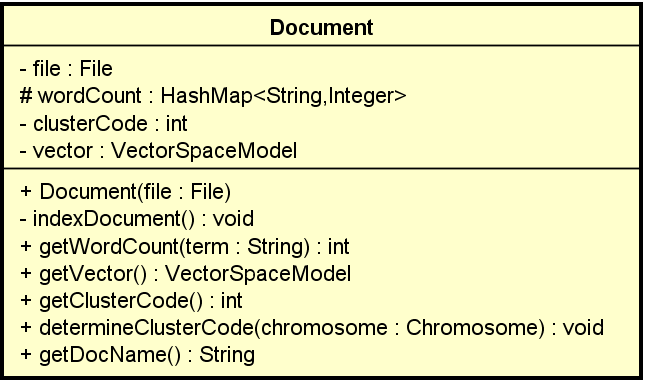
\includegraphics[width=0.5\textwidth]{DiagramKelas/Document}
		\caption{Kelas \textit{Document}}
		\label{fig:kelasDocument}
	\end{center}
\end{figure}

Kelas ini merupakan representasi dari dokumen yang akan diproses dalam pengelompokan. Kelas ini berfungsi untuk menyimpan informasi yang dibutuhkan dari sebuah dokumen selama proses pengelompokan. Atribut yang dimiliki oleh kelas \textit{Document} adalah:

\begin{itemize}
	\item \textit{wordCount}: bertipe \textit{HashMap} dengan \textit{key} bertipe \textit{String} dan \textit{value} bertipe \textit{Integer}. Atribut ini menyimpan pasangan kata yang dimiliki oleh dokumen tersebut dan frekuensinya.
	\item \textit{file}: atribut ini bertipe \textit{File} milik \textit{package} java.io yang berfungsi untuk merepresentasikan \textit{file} dari dokumen yang akan diproses.
	\item \textit{vector}: atribut bertipe \textit{VectorSpaceModel} ini merepresentasikan model ruang vektor pada sebuah dokumen.
\end{itemize}

\textit{Method} yang terdapat dalam kelas ini adalah:

\begin{itemize}
	\item \textit{Document}: merupakan \textit{constructor} dengan sebuah parameter bertipe \textit{File} yaitu \textit{file} dari dokumen yang akan dikelompokkan.
	\item \textit{indexDocument}: \textit{method} tanpa kembalian (\textit{void}) yang berfungsi untuk mengindeks dokumen untuk mengisi atribut \textit{wordCount}.
	\item \textit{getWordCount}: berfungsi untuk mengembalikan banyaknya istilah \textit{term} muncul dalam dokumen.
	\item \textit{getVector}: merupakan \textit{getter} dari variabel \textit{vector}.
	\item \textit{determineClusterCode}: berfungsi untuk menentukan \textit{cluster} dari dokumen.
	\item \textit{getDocName}: mengembalikan nama \textit{file} dari dokumen.
\end{itemize}

\subsubsection*{\textit{VectorSpaceModel}}

\begin{figure}[h]
	\begin{center}
		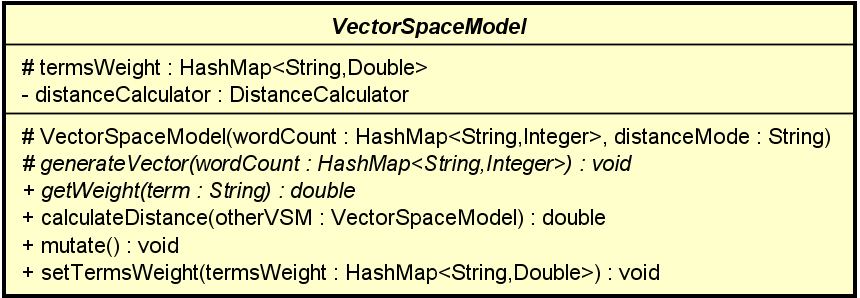
\includegraphics[width=0.5\textwidth]{DiagramKelas/VectorSpaceModel}
		\caption{Kelas \textit{VectorSpaceModel}}
		\label{fig:kelasVSM}
	\end{center}
\end{figure}

Kelas ini merupakan kelas abstrak yang merepresentasikan model ruang vektor. kelas ini memiliki fungsi-fungsi yang umum dimiliki oleh sebuah model ruang vektor. Atribut yang dimiliki kelas ini adalah:

\begin{itemize}
	\item \textit{termsWeight}: bertipe \textit{Hashmap} dengan \textit{key} berupa \textit{String} dan \textit{value} berupa \textit{Double}. atribut ini menyimpan pasangan istilah dan bebatnya sesuai dengan metode pembobotan.
	\item \textit{distanceCalculator}: bertipe \textit{DistanceCalculator} dan merupakan objek yang akan digunakan untuk menghitung jarak antar vektor.
\end{itemize}

\textit{Method} yang terdapat dalam kelas ini adalah:

\begin{itemize}
	\item \textit{VectorSpaceModel}: merupakan constructor dengan dua parameter yaitu \textit{wordCount} bertipe \textit{Hashmap<String,Integer>} yang merupakan pasangan kata dan banyak kemunculannya dalam dokumen serta \textit{distanceMode} bertipe \textit{String} yang akan menentukan tipe perhitungan jarak antar vektor.
	\item \textit{generateVector}: merupakan \textit{method} tanpa parameter untuk mengubah banyak kemunculan kata menjadi berat.
	\item \textit{getWeight}: berfungsi untuk mengembalikan berat dari istilah \textit{term}.
	\item \textit{calculateDistance}: berfungsi untuk menghitung jarak antara vektor ini dengan \textit{otherVSM} menggunakan metode yang dipilih pada parameter di \textit{constructor}.
	\item \textit{mutate}: merupakan \textit{method} untuk melakukan mutasi pada sebuah dimensi dalam vektor.
	\item \textit{setTermsWeight}: merupakan setter dari atribut \textit{termsWeight}.
\end{itemize}

\subsubsection*{\textit{BagOfWordVSM}}

\begin{figure}[h]
	\begin{center}
		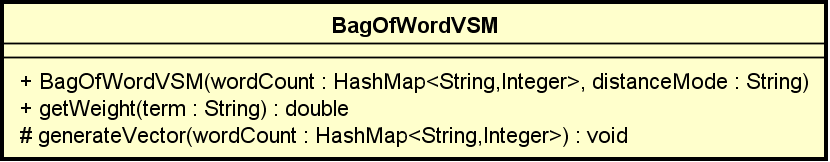
\includegraphics[width=0.5\textwidth]{DiagramKelas/BagOfWordVSM}
		\caption{Kelas \textit{BagOfWordVSM}}
		\label{fig:kelasBagOfWordVSM}
	\end{center}
\end{figure}

Kelas ini merupakan kelas yang mengimplementasikan kelas \textit{VectorSpaceModel}. Kelas ini menggunakan metode pembobotan \textit{BagOfWord} di mana bobot tiap istilah merupakan banyaknya kemunculan istilah itu sendiri. Atribut yang dimiliki kelas ini seluruhnya merupakan atribut yang diturunkan dari kelas \textit{VectorSpaceModel} dan hanya melakukan \textit{override} pada \textit{method} yang masih bersifat abstrak.

\subsubsection*{\textit{DistanceCalculator}}

\begin{figure}[h]
	\begin{center}
		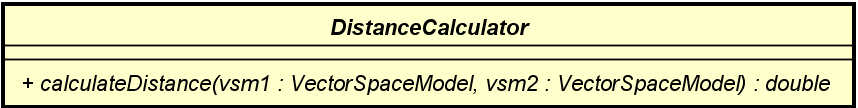
\includegraphics[width=0.5\textwidth]{DiagramKelas/DistanceCalculator}
		\caption{Kelas \textit{DistanceCalculator}}
		\label{fig:kelasDistanceCalculator}
	\end{center}
\end{figure}

Kelas ini merupakan kelas abstrak yang berfungsi untuk menghitung jarak antara dua buah objek bertipe \textit{VectorSpaceModel}. Kelas ini tidak memiliki atribut dan hanya memiliki sebuah \textit{method} abstrak yaitu \textit{calculateDistance} yang memiliki dua buah parameter \textit{vsm1} dan \textit{vsm2}. Hasil yang dikembalikan oleh \textit{method} ini adalah jarak dari kedua vektor tersebut sesuai dengan metode perhitungan jaraknya.

\subsubsection*{\textit{EuclideanDistanceCalculator}}

\begin{figure}[h]
	\begin{center}
		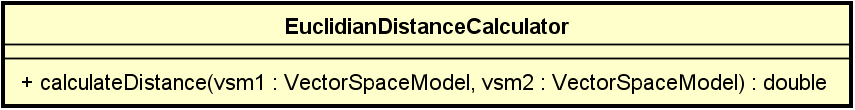
\includegraphics[width=0.5\textwidth]{DiagramKelas/EuclideanDistanceCalculator}
		\caption{Kelas \textit{EuclideanDistanceCalculator}}
		\label{fig:kelasEuclideanDist}
	\end{center}
\end{figure}

Kelas ini mengimplementasikan kelas abstrak \textit{DistanceCalculator}. Kelas ini hanya melakukan \textit{override} pada \textit{method calculateDistance} dengan melakukan perhitungan menggunakan jarak euclidean untuk menghitung jarak antara dua buah vektor (Subbab \ref{sub:euclideanDist}).

\subsubsection*{\textit{CosineDistanceCalculator}}

\begin{figure}[h]
	\begin{center}
		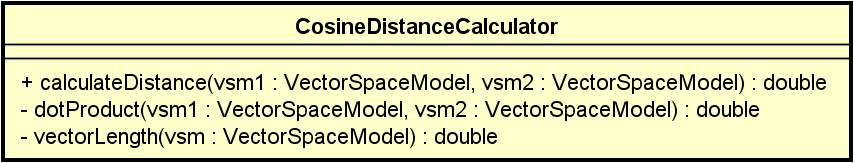
\includegraphics[width=0.5\textwidth]{DiagramKelas/CosineDistanceCalculator}
		\caption{Kelas \textit{CosineDistanceCalculator}}
		\label{fig:kelasCosineDist}
	\end{center}
\end{figure}

Kelas ini juga mengimplementasikan kelas abstrak \textit{DistanceCalculator}. Kelas ini memiliki dua \textit{method} tambahan selain melakukan \textit{override} pada \textit{method calculateDistance}. \textit{Method} yang ada pada kelas ini adalah:

\begin{itemize}
	\item \textit{calculateDistance}: merupakan \textit{method} yang diturunkan dari kelas \textit{DistanceCalculator}. \textit{Method} ini mengembalikan jarak dari \textit{vsm1} dan \textit{vsm2} yang dihitung menggunakan persamaan cosinus (Subbab \ref{sub:cosineDist}).
	\item \textit{dotProduct}: berfungsi untuk menghitung hasil perkalian titik (\textit{dot product}) antara \textit{vsm1} dan \textit{vsm 2}.
	\item \textit{vectorLength}: berfungsi untuk menghitung panjang dari vektor \textit{vsm}.
\end{itemize}

\subsubsection*{\textit{Dictionary}}

\begin{figure}[h]
	\begin{center}
		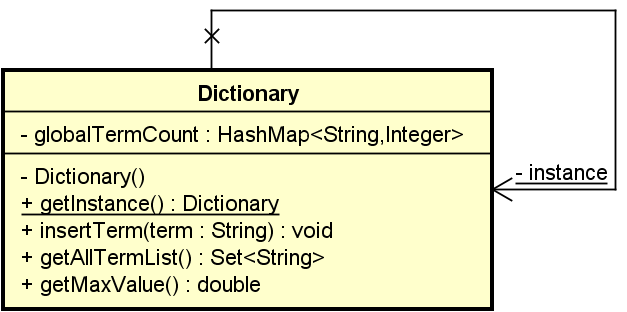
\includegraphics[width=0.5\textwidth]{DiagramKelas/Dictionary}
		\caption{Kelas \textit{Dictionary}}
		\label{fig:kelasDictionary}
	\end{center}
\end{figure}

Kelas ini merepresentasikan sebuah kamus yang menangani seluruh kebutuhan dalam proses pengelompokan yang membutuhkan akses global untuk keseluruhan koleksi dokumen. Atribut yang ada dalam kelas ini adalah:

\begin{itemize}
	\item \textit{globalTermCount}: bertipe \textit{HashMap} dengan \textit{key} bertipe \textit{String} dan \textit{value} bertipe \textit{Integer}. Atribut ini berfungsi untuk menyimpan seluruh istilah yang muncul dan banyak kemunculannya dalam keseluruhan koleksi dokumen.
	\item \textit{instance}: merupakan objek bertipe \textit{Dictionary} sebagai instansiasi satu-satunya dari kelas \textit{Dictionary} karena kelas ini bersifat \textit{singleton}.
\end{itemize}

\textit{Method} yang ada pada kelas ini adalah:

\begin{itemize}
	\item \textit{Dictionary}: merupakan \textit{constructor private} untuk menjamin tidak akan ada lebih dari satu \textit{instance} selama perangkat lunak berjalan.
	\item \textit{getInstance}: merupakan \textit{method static} yang berfungsi sebagai \textit{getter} dari atribut \textit{instance}.
	\item \textit{insertTerm}: berfungsi untuk memasukkan istilah \textit{term} ke dalam variabel \textit{globalTermCount}.
	\item \textit{getAllTermList}: bertugas mengembalikan daftar seluruh istilah yang pernah muncul di seluruh koleksi dokumen.
	\item \textit{getValue}: bertugas mengembalikan banyaknya kata \textit{term} muncul dalam seluruh koleksi dokumen. 
\end{itemize}

\subsubsection*{\textit{Gene}}

\begin{figure}[h]
	\begin{center}
		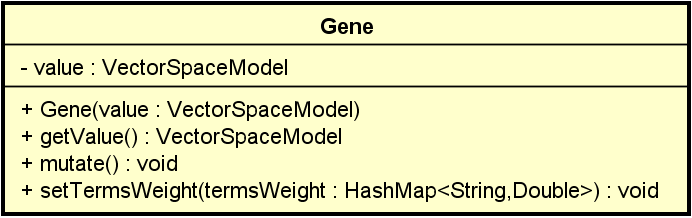
\includegraphics[width=0.5\textwidth]{DiagramKelas/Gene}
		\caption{Kelas \textit{Gene}}
		\label{fig:kelasGene}
	\end{center}
\end{figure}

Kelas ini merepresentasikan gen dalam algoritma genetika. Kelas ini hanya memiliki sebuah atribut \textit{value} bertipe \textit{VectorSpaceModel}. Atribut ini menyimpan model ruang vektor yang menjadi titik pusat \textit{cluster} (\textit{centroid}). \textit{Method} yang ada pada kelas ini adalah:

\begin{itemize}
	\item \textit{Gene}: merupakan \textit{constructor} dari kelas \textit{Gene} yang membutuhkan sebuah parameter bertipe \textit{VectorSpaceModel} untuk mengisi variabel \textit{value}.
	\item \textit{getValue}: merupakan \textit{getter} dari atribut \textit{value}.
	\item \textit{mutate}: berfungsi untuk melakukan mutasi pada gen. \textit{Method} ini sebenarnya hanya bertugas memanggil fungsi \textit{mutate()} dari atribut \textit{value}.
	\item \textit{setTermsWeight}: berfungsi untuk mengubah nilai atribut \textit{termsWeight} milik atribut \textit{value}.
\end{itemize}

\subsubsection*{\textit{Chromosome}}

\begin{figure}[h]
	\begin{center}
		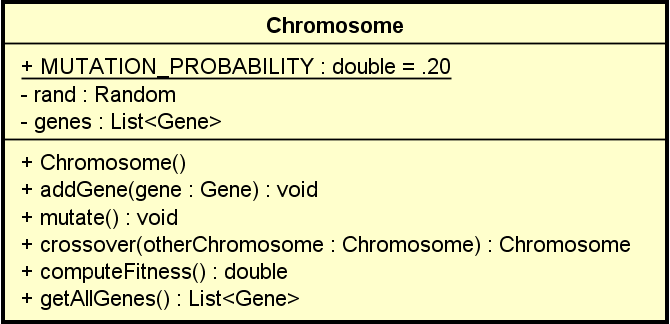
\includegraphics[width=0.5\textwidth]{DiagramKelas/Chromosome}
		\caption{Kelas \textit{Chromosome}}
		\label{fig:kelasChromosome}
	\end{center}
\end{figure}

Kelas ini merepresentasikan kromosom dalam algoritma genetika (Subbab \ref{sub:chromosome}). Atribut yang terdapat dalam kelas ini adalah:

\begin{itemize}
	\item \textit{genes}: bertipe \textit{List of Gene} dan merupakan kumpulan gen yang terdapat dalam kromosom.
	\item \textit{MUTATION\_ PROBABILITY}: merupakan atribut yang bersifat \textit{static} dan \textit{final} yang berisi probabilitas terjadinya mutasi dalam proses pembangkitan keturunan.
\end{itemize}

\textit{Method} yang terdapat dalam kelas ini adalah:

\begin{itemize}
	\item \textit{Chromosome}: merupakan \textit{constructor} tanpa parameter untuk membentuk objek dari kelas \textit{Chromosome}.
	\item \textit{addGene}: bertugas untuk menambahkan satu gen ke dalam kromosom (ke dalam atribut \textit{genes}).
	\item \textit{mutate}: berfungsi untuk melakukan mutasi pada kromosom dengan cara melakukan mutasi pada sebuah gen secara acak (Subbab \ref{sub:mutation}).
	\item \textit{crossover}: bertugas untuk melakukan persilangan dengan kromosom lain untuk mengahsilkan keturunan (Subbab \ref{sub:crossover}).
	\item \textit{computeFitness}: mengembalikan nilai \textit{fitness} dari kromosom (Subbab \ref{sub:fitnessFn}).
	\item \textit{getAllGenes}: merupakan \textit{getter} dari atribut \textit{genes}.
\end{itemize}

\subsubsection*{\textit{Clusterer}}

\begin{figure}[h]
	\begin{center}
		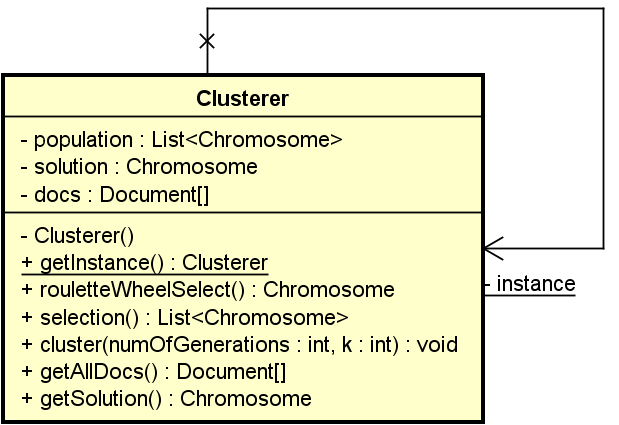
\includegraphics[width=0.5\textwidth]{DiagramKelas/Clusterer}
		\caption{Kelas \textit{Clusterer}}
		\label{fig:kelasClusterer}
	\end{center}
\end{figure}

Kelas ini merupakan kelas utama yang akan mengatur jalannya proses pengelompokan. Kelas ini merupakan kelas singleton. Atribut yang terdapat dalam kelas ini adalah:

\begin{itemize}
	\item \textit{docs}: bertipe \textit{List of Document} yang berfungsi untuk menyimpan seluruh koleksi dokumen.
	\item \textit{instance}: variabel \textit{static} ini berfungsi untuk menyimpan \textit{instance} dari kelas \textit{Clusterer}.
	\item \textit{population}: bertipe \textit{List of Chromosome} yang merepresentasikan populasi pada generasi saat ini.
	\item \textit{solution}: bertipe \textit{Chromosome} yang mencatat kromosom dengan nilai \textit{fitness} terbaik.
\end{itemize}

\textit{Method} yang terdapat dalam kelas ini adalah:

\begin{itemize}
	\item \textit{Clusterer}: merupakan \textit{constructor private} yang berfungsi untuk menjamin tidak akan ada \textit{instance} dibuat diluar dari kelas ini.
	\item \textit{getInstance}: merupakan \textit{getter} dari variabel \textit{instance}.
	\item \textit{rouletteWheelSelect}: bertugas untuk memilih dua kromosom dan melakukan persilangan untuk menghasilkan sebuah keturunan selanjutnya.
	\item \textit{selection}: bertugas untuk melakukan \textit{roulette wheel selection} sebanyak populasi untuk menghasilkan populasi dari generasi selanjutnya.
	\item \textit{cluster}: merupakan \textit{method} utama yang bertugas melakukan pengelompokan dokumen dengan dua parameter yaitu jumlah generasi dan nilai $k$.
	\item \textit{getAllDocs}: merupakan \textit{getter} dari atribut \textit{docs}.
	\item \textit{getSolution}: merupakan \textit{getter} dari atribut \textit{solution}.
\end{itemize}

\begin{figure}
	\begin{center}
		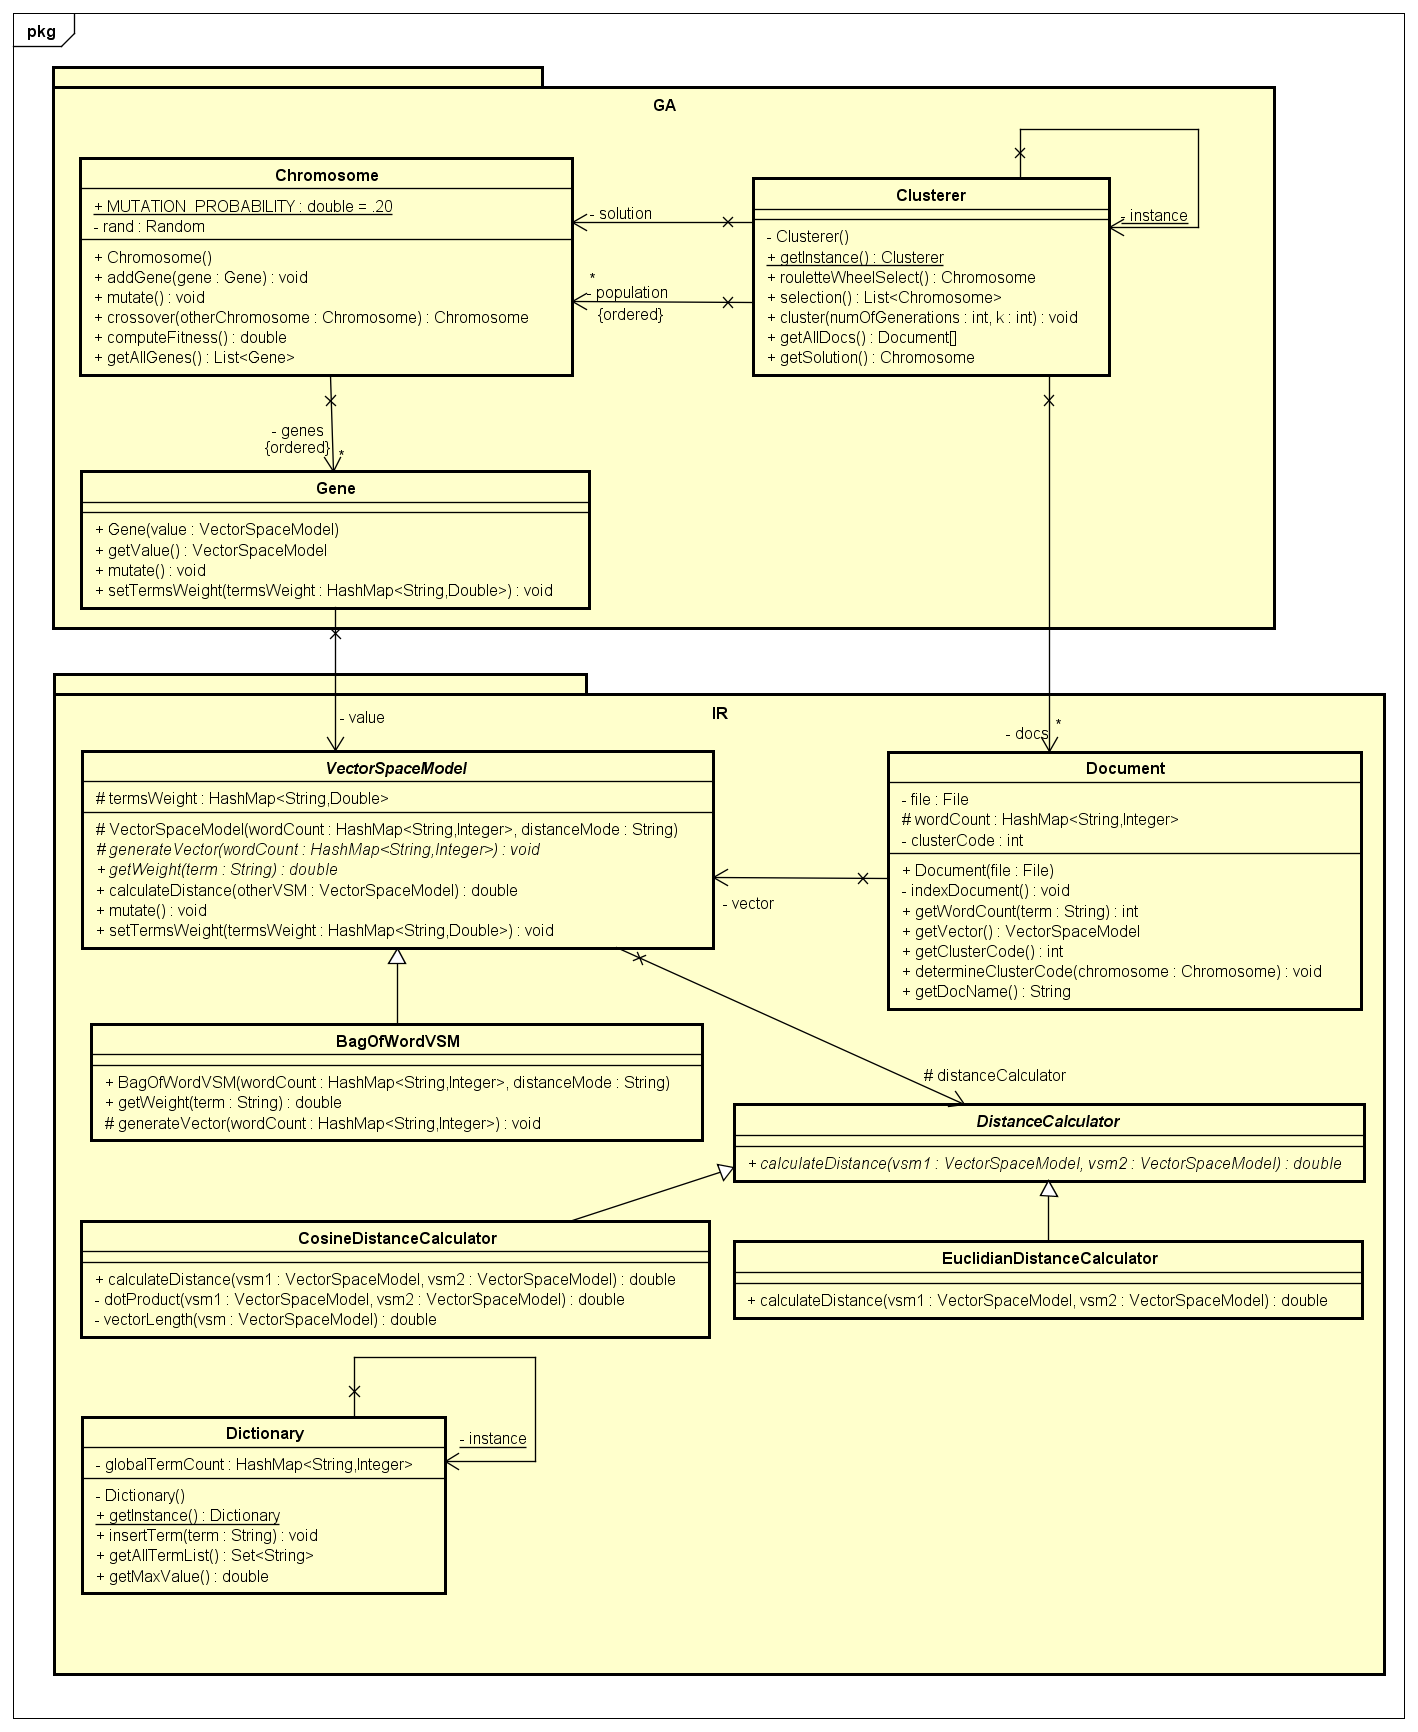
\includegraphics[width=\textwidth]{DiagramKelas}
		\caption{Diagram kelas pada tahap perancangan}
		\label{fig:diagramkelas}
	\end{center}
\end{figure}

\newpage

\subsection*{Perancangan Antarmuka Pengguna}
Antarmuka yang dirancang untuk perangkat lunak ini hanya terdiri dari satu jendela utama dan dua jendela \textit{pop-up}. Pada penelitian ini, perancangan antarmuka dibuat menggunakan perangkat lunak \textit{balsamiq}\footnote{https://balsamiq.com/}. Setiap objek dan \textit{field} akan diberi label unik agar dapat disesuaikan dengan tabel keterangan. Berikut akan dibahas rancangan antarmuka pengguna dari perangkat ini.

\subsubsection*{Jendela Utama}
Gambar \ref{fig:UIUtama} merupakan jendela yang pertama kali ditampilkan saat perangkat lunak dijalankan. Jendela tersebut berisi berbagai macam hal yang dibutuhkan penguna dalam melakukan pengelompokan dokumen. 

\begin{figure}[h]
	\begin{center}
		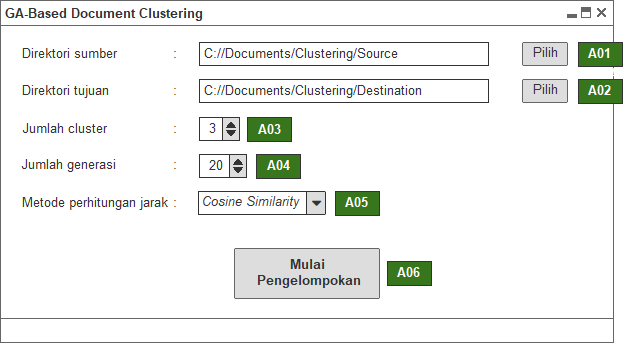
\includegraphics[width=0.7\textwidth]{UI/Main}
		\caption{Rancangan antarmuka jendela utama}
		\label{fig:UIUtama}
	\end{center}
\end{figure}

Penjelasan setiap \textit{field} dalam jendela utama adalah sebagai berikut:

\begin{table}[h]
	\label{tbl:fieldUtama}
	\renewcommand{\arraystretch}{2}
	\begin{tabularx}{\textwidth}{l X l X l X} \hline
		\textbf{Kode} & \textbf{Nama} & \textbf{Jenis} & \textbf{\textit{Defaut value}} & \textbf{Wajib} & \textbf{Aturan validasi} \\ \hline
		A01 & Direktori sumber & \textit{file chooser} & - & ya & Harus berupa direktori yang berisi dokumen (tidak boleh kosong) \\ \hline
		A02 & Direktori tujuan & \textit{file chooser} & - & ya & Harus berupa direktori yang kosong \\ \hline
		A03 & Jumlah cluster & \textit{spinner} & 2 & ya & Nilai minimum 2 \\ \hline
		A04 & Jumlah generasi & \textit{spinner} & 1 & ya & Nilai minimum 1 \\ \hline
		A05 & Metode perhitungan jarak & \textit{dropdown} & \textit{Cosine Similarity} & ya & - \\ \hline
	\end{tabularx}
	\caption{Rincian \textit{field} pada jendela utama}
\end{table}

Jendela ini hanya memiliki sebuah tombol dengan kode \textbf{A06} yang berfungsi untuk memulai proses pengelompokan dan membuka jendela \textit{loading}. Selain tombol, pada jendela ini juga terdapat lima \textit{field} seperti yang tertera pada Tabel \ref{tbl:fieldUtama}.

\subsubsection*{Jendela \textit{Loading}}

\begin{figure}[h]
	\begin{center}
		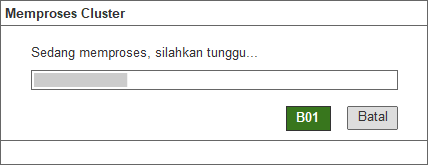
\includegraphics[width=0.7\textwidth]{UI/LoadingPage}
		\caption{Rancangan antarmuka jendela \textit{loading}}
		\label{fig:UILoading}
	\end{center}
\end{figure}

Gambar \ref{fig:UILoading} merupakan jendela yang akan muncul setelah pengguna menekan tombol "Mulai Pengelompokan". Jendela ini berisi informasi perkembangan proses pengelompokan. Informasi ini disajikan dalam bentuk \textit{progress bar}. Hanya ada sebuah tombol pada jendela ini yaitu tombol dengan kode \textbf{B01}. Sesuai dengan labelnya, tombol ini berfungsi untuk membatalkan proses pengelompokan. Apabila tombol batal ditekan, maka pengguna akan dikembalikan ke jendela utama (Gambar \ref{fig:UIUtama}).

\subsubsection*{Jendela Proses Berhasil}
\begin{figure}[h]
	\begin{center}
		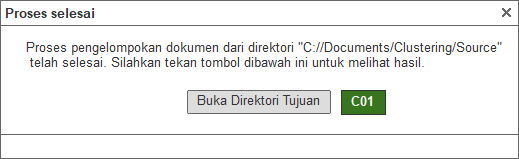
\includegraphics[width=0.7\textwidth]{UI/Output}
		\caption{Rancangan antarmuka jendela proses berhasil}
		\label{fig:UISuccess}
	\end{center}
\end{figure}

Gambar \ref{fig:UISuccess} akan ditampilkan setelah proses pengelompokan berhasil, yaitu saat \textit{progress bar} di jendela \textit{loading} sudah terisi penuh. Jendela ini hanya memiliki satu buah tombol yaitu tombol dengan kode \textbf{C01} yang berfungsi untuk membuka \textit{Windows Explorer} pada direktori hasil yang sudah dipilih pengguna pada jendela utama untuk menampilkan hasil dari proses pengelompokan.

		\item \textbf{Mengimplementasikan hasil rancangan menjadi perangkat lunak.}\\
    	{\bf Status :} Ada sejak rencana kerja skripsi\\
		{\bf Hasil :} Hasil implementasi dilampirkan.
	\end{enumerate}

\section{Pencapaian Rencana Kerja}
Langkah-langkah kerja yang berhasil diselesaikan dalam Skripsi 1 ini adalah sebagai berikut:
\begin{enumerate}
	\item Melakukan studi literatur mengenai {\it Information Retrieval} (temu kembali informasi).
	\item Melakukan studi literatur mengenai {\it Document Clustering} (pengelompokan dokumen).
    \item Melakukan studi literatur mengenai {\it Genetic Algorithm} (algoritma genetik).
    \item Mempelajari penggunaan algoritma genetik dalam pengelompokan dokumen.
    \item Melakukan analisis masalah dan mencari solusinya.
    \item Membuat rancangan perangkat lunak yang menggunakan algoritma genetik sebagai algoritma pengelompokan dokumen.
    \item Mengimplementasikan hasil rancangan menjadi perangkat lunak.
\end{enumerate}


\section{Kendala yang Dihadapi}
%TULISKAN BAGIAN INI JIKA DOKUMEN ANDA TIPE A ATAU C
Kendala - kendala yang dihadapi selama mengerjakan skripsi :
\begin{itemize}
	\item Skripsi 1 diambil bersamaan dengan Skripsi 2 sehingga waktu yang tersedia sangat terbatas sedangkan banyak hal yang perlu dikerjakan.
	\item Ada beberapa tugas besar dari mata kuliah lain yang menyita cukup banyak waktu sehingga mengurangi waktu untuk mengerjakan skripsi.
\end{itemize}

\vspace{1cm}
\centering Bandung, \tanggal\\
\vspace{2cm} \nama \\ 
\vspace{1cm}

Menyetujui, \\
\ifdefstring{\jumpemb}{2}{
\vspace{1.5cm}
\begin{centering} Menyetujui,\\ \end{centering} \vspace{0.75cm}
\begin{minipage}[b]{0.45\linewidth}
% \centering Bandung, \makebox[0.5cm]{\hrulefill}/\makebox[0.5cm]{\hrulefill}/2013 \\
\vspace{2cm} Nama: \pembA \\ Pembimbing Utama
\end{minipage} \hspace{0.5cm}
\begin{minipage}[b]{0.45\linewidth}
% \centering Bandung, \makebox[0.5cm]{\hrulefill}/\makebox[0.5cm]{\hrulefill}/2013\\
\vspace{2cm} Nama: \pemB \\ Pembimbing Pendamping
\end{minipage}
\vspace{0.5cm}
}{
% \centering Bandung, \makebox[0.5cm]{\hrulefill}/\makebox[0.5cm]{\hrulefill}/2013\\
\vspace{2cm} Nama: \pembA \\ Pembimbing Tunggal
}

\newpage
\section*{Lampiran Kode Program}
 
\lstset{numbers=left,stepnumber=1, numbersep=5pt, frame=leftline,
	tabsize=4, breaklines=true, basicstyle=\fontfamily{fvm}\selectfont\tiny, 
	commentstyle=\itshape\color{gray}, keywordstyle=\bfseries\color{blue}, 
	identifierstyle=\color{black}, stringstyle=\color{orange},
	literate={-}{-}1{-\,-}{--}1
} 

\lstinputlisting[language=Java, caption=Chromosome.java]{src/GA/Chromosome.java}
\lstinputlisting[language=Java, caption=Clusterer.java]{src/GA/Clusterer.java}
\lstinputlisting[language=Java, caption=Gene.java]{src/GA/Gene.java}
\lstinputlisting[language=Java, caption=BagOfWordVSM.java]{src/IR/BagOfWordVSM.java}
\lstinputlisting[language=Java, caption=CosineDistanceCalculator.java]{src/IR/CosineDistanceCalculator.java}
\lstinputlisting[language=Java, caption=Dictionary.java]{src/IR/Dictionary.java}
\lstinputlisting[language=Java, caption=DistanceCalculator.java]{src/IR/DistanceCalculator.java}
\lstinputlisting[language=Java, caption=Document.java]{src/IR/Document.java}
\lstinputlisting[language=Java, caption=EuclidianDistanceCalculator.java]{src/IR/EuclidianDistanceCalculator.java}
\lstinputlisting[language=Java, caption=VectorSpaceModel.java]{src/IR/VectorSpaceModel.java}

\end{document}

